\documentclass{article}

\usepackage{microtype}
\usepackage{graphicx}
\usepackage{booktabs}
\usepackage{hyperref}

% Anonymous workshop format by default.
\usepackage{icml2026}

\usepackage{amsmath,amssymb,amsthm,mathtools}
\usepackage{enumitem}
\usepackage[capitalize,noabbrev]{cleveref}
\crefname{assumption}{Assumption}{Assumptions}
\Crefname{assumption}{Assumption}{Assumptions}

\theoremstyle{plain}
\newtheorem{theorem}{Theorem}[section]
\newtheorem{lemma}[theorem]{Lemma}
\newtheorem{proposition}[theorem]{Proposition}
\newtheorem{corollary}[theorem]{Corollary}
\theoremstyle{definition}
\newtheorem{assumption}{Assumption}
\newtheorem{definition}[theorem]{Definition}
\theoremstyle{remark}
\newtheorem{remark}[theorem]{Remark}

\newcommand{\E}{\mathbb{E}}
\newcommand{\R}{\mathbb{R}}
\newcommand{\K}{\mathcal{K}}
\newcommand{\B}{\mathcal{B}}
\newcommand{\N}{\mathcal{N}}
\newcommand{\F}{\mathcal{F}}
\newcommand{\dist}{\operatorname{dist}}
\newcommand{\Proj}{\operatorname{Proj}}
\newcommand{\Var}{\operatorname{Var}}
\newcommand{\diag}{\operatorname{diag}}

\icmltitlerunning{Meta-MAPG as Stochastic Approximation}

\begin{document}

\twocolumn[
\icmltitle{Opponent-Aware Policy Gradient as Stochastic Approximation: Local Meta-MAPG Convergence and Restart Globalisation}

\begin{icmlauthorlist}
\icmlauthor{Anonymous Author}{anon}
\end{icmlauthorlist}

\icmlaffiliation{anon}{Anonymous Institution}
\icmlcorrespondingauthor{Anonymous Author}{anonymous@icml.cc}
\icmlkeywords{multi-agent reinforcement learning, stochastic games, policy gradient, opponent shaping}

\vskip 0.3in
]

\printAffiliationsAndNotice{}

\begin{abstract}
Policy-gradient methods in general stochastic games admit local convergence guarantees near stable Nash policies, but these guarantees are usually stated for independent policy-gradient fields that do not anticipate opponent learning. Opponent-aware methods such as LOLA and Meta-MAPG add terms that differentiate through the future learning of other agents, and empirically change both adaptation and equilibrium selection. We analyze this mechanism through a two-phase stochastic-approximation scheme. In the first phase, a constant Meta-MAPG correction is used to enter the basin of a stable Nash equilibrium more quickly; when the shaped field improves the local drift by $\lambda\mu_M$, the required basin-entry time decreases by the same factor. In the second phase, the shaping coefficient is annealed to zero, so Giannou et al.'s local convergence theorem applies near strategically stable Nash equilibria of the original game. Independent restarts then turn the local result into an almost-sure finite-restart guarantee with a geometric tail bound. Small tabular experiments match the main theoretical claims: peer-learning terms change equilibrium selection, larger restart budgets improve selection outcomes, basin maps expand under opponent-aware shaping, and estimator variance decreases with batch size.
\end{abstract}

\section{Introduction}

Learning in stochastic games is hard because each learner faces both an evolving environment and other learners whose policies change in response to the same data. Recent work by \citet{giannou2022convergence} showed that policy-gradient methods converge locally to stable Nash policies in general stochastic games under strategic stability and second-order sufficiency conditions. This result is a strong baseline, but the update it analyses treats opponent learning as part of the background stochastic process rather than as an object to be shaped.

Opponent-aware policy gradients address this missing dependence. LOLA differentiates through an opponent's anticipated update \citep{foerster2018lola,letcher2019stable}. Meta-MAPG derives a meta-policy-gradient theorem with three terms: the current-policy gradient, an own-learning gradient, and a peer-learning gradient that captures how the agent's current behaviour changes the future policies of other agents \citep{kim2021meta}. These terms matter empirically, but the convergence status of the resulting stochastic process is less clear than for standard PG.

We close this gap in three steps. First, under bounded rewards, smooth policies, controlled unroll length, and standard sampling assumptions, we show that the Meta-MAPG update is a stochastic approximation to the base game-gradient field plus controlled opponent-aware terms. Second, we prove a two-phase result that separates the short-run use of constant shaping from the asymptotic need for annealing. Constant Meta-MAPG shaping is used only for a finite basin-entry phase; once the iterate reaches a safe subset of the stable basin, the shaping coefficient is annealed so that the limiting stationary points remain the stable Nash equilibria of the original stochastic game.

Third, we extend the local theorem with independent restarts. Local convergence still depends on the basin of attraction; even normal-form games can contain cycles and multiple attractors. If restarts draw from a full-support distribution on a compact policy-parameter set, however, each epoch has a fixed positive probability of starting in the local basin. This yields an almost-sure finite-restart guarantee and an explicit expected restart bound. In this setting, restart budget becomes a simple equilibrium-selection mechanism whose effect is governed by basin mass. Experiments in Stag Hunt and iterated Prisoner's Dilemma are designed to match the theorem's ingredients: component ablations, restart-budget selection, basin volume, and estimator variance.

\paragraph{Positioning.}
This paper is complementary to prior opponent-shaping algorithms. LOLA introduced differentiating through an opponent update \citep{foerster2018lola}; SOS stabilised opponent shaping in differentiable games \citep{letcher2019stable}; COLA addresses consistency of mutual shaping \citep{willi2022cola}; POLA improves parameterisation behaviour via a proximal view \citep{zhao2022pola}; and M-FOS learns long-horizon shaping policies without a differentiable opponent model \citep{lu2022mfos}. Our question is narrower: when can a finite-unroll Meta-MAPG estimator be analysed within stochastic approximation and used to improve basin entry without changing the asymptotic Nash target?

\begin{table}[t]
  \centering
  \caption{Positioning among opponent-aware methods. ``Nash-preserving'' means the stated theory preserves the original game's stable Nash target rather than merely optimising a shaped meta-objective.}
  \label{tab:related}
  \resizebox{\linewidth}{!}{
  \begin{tabular}{lcccc}
  \toprule
  Method & Convergence & Shaping & Opp. model & Nash-pres.\\
  \midrule
  LOLA & No general & 1-step gradient & White-box & No\\
  SOS & Differentiable games & Stable OS & White-box & SFP-focused\\
  COLA & Simple-game stability & Consistent OS & White-box & No\\
  POLA & Empirical/proximal & Proximal OS & Learned & Not primary\\
  M-FOS & Empirical & Meta-policy OS & No & No\\
  This work & Local SA + restarts & Two-phase Meta-MAPG & Sample estimates & Yes, by annealing\\
  \bottomrule
  \end{tabular}}
\end{table}

\section{Setup}\label{sec:setup}

\subsection{Stochastic Games}

We consider finite discounted stochastic games
\[
\mathcal{G}=(N,\mathcal{S},\{\mathcal{A}_i\}_{i\in N},P,\{r_i\}_{i\in N},\rho,\gamma_{\mathrm{disc}}),
\]
with finite state space $\mathcal{S}$, finite action sets $\mathcal{A}_i$, transition kernel $P$, bounded rewards $|r_i|\le R_{\max}$, initial-state distribution $\rho$, and discount factor $\gamma_{\mathrm{disc}}\in[0,1)$. Each agent has a differentiable stationary Markov policy $\pi_{\phi_i}(a_i\mid s)$ with parameter $\phi_i\in\R^{d_i}$; the joint parameter is $\phi=(\phi_i)_{i=1}^N\in\R^d$. The value of agent $i$ is
\[
J_i(\phi)=\E_{\rho,\pi_\phi}\!\left[\sum_{t\ge 0}\gamma_{\mathrm{disc}}^t r_i(s_t,a_t)\right],
\]
and the standard game-gradient field is
\[
v(\phi)=\bigl(\nabla_{\phi_i}J_i(\phi)\bigr)_{i=1}^N.
\]
First-order stationary points of this field correspond to Nash policies under the gradient-dominance property used by \citet{giannou2022convergence}; finite stochastic games possess stationary Nash equilibria \citep{fink1964equilibrium}.

\begin{definition}[Stable Nash and SOS]\label{def:sos}
A Nash parameter $\phi^\ast$ is stable if
\[
\langle v(\phi),\phi-\phi^\ast\rangle <0
\]
for all $\phi\ne\phi^\ast$ sufficiently close to $\phi^\ast$. It is second-order stationary (SOS) if there exist $\mu>0$ and $\rho>0$ such that
\[
\langle v(\phi),\phi-\phi^\ast\rangle\le -\mu\|\phi-\phi^\ast\|^2
\]
whenever $\|\phi-\phi^\ast\|\le\rho$.
\end{definition}

The SOS condition is the quantitative stability condition that yields an attracting neighbourhood and a rate in \citet{giannou2022convergence}. We use it as the local anchor.

\subsection{Meta-MAPG Field}

Meta-MAPG views learning as a Markov chain of joint policy parameters $\phi_0,\ldots,\phi_L$, where each inner transition is produced by a policy-gradient update. For agent $i$, \citet{kim2021meta} decompose the meta-gradient into
\[
G_i^{\mathrm{MAPG}}
=G_i^{\mathrm{cur}}+G_i^{\mathrm{own}}+G_i^{\mathrm{peer}}.
\]
The current term is the usual policy-gradient score term. The own-learning term differentiates through how $\phi_i^0$ affects agent $i$'s adapted parameters $\phi_i^{1:L}$. The peer-learning term differentiates through how $\phi_i^0$ affects other agents' future parameters $\phi_{-i}^{1:L}$. The peer term is the Meta-MAPG analogue of LOLA-style opponent shaping; the own term is absent from pure LOLA.

We write the population opponent-aware field as
\[
F_L(\phi)=v(\phi)+M_L^{\mathrm{own}}(\phi)+M_L^{\mathrm{peer}}(\phi),
\]
where $L$ is the unroll length. In the convergence theorem we use the annealed update
\begin{equation}\label{eq:update}
\phi_{n+1}
=\Proj_{\K}\!\left[\phi_n+\alpha_n\left(\hat v_n+\lambda_n\hat M_{L_n,n}\right)\right],
\end{equation}
where $\K\subset\R^d$ is compact, $\hat M_{L_n,n}$ estimates the combined own/peer Meta-MAPG correction, and $\lambda_n$ controls the asymptotic size of opponent-aware shaping. The compact projection can be replaced by any standard boundedness mechanism; it is stated explicitly so that the projection lemma of \citet{kushner1978stochastic} applies and so that the ODE tracking argument in \citet{borkar2008stochastic} holds without additional tightness work.

\begin{definition}[Nash-consistent shaping]\label{def:nash-consistent}
Let $U$ be a neighbourhood of a stable Nash set $\N$ of the base game-gradient field $v$. A scheduled opponent-aware correction $\lambda_n M_{L_n}$ is Nash-consistent on $U$ if its contribution to the stochastic-approximation recursion is either summable,
\[
\sup_{\phi\in U}\|\lambda_n M_{L_n}(\phi)\|\le \beta_n,
\qquad \sum_n \alpha_n\beta_n<\infty,
\]
so the limiting ODE on $U$ is $\dot\phi=v(\phi)$, or else its non-vanishing limit field $v+M$ has exactly the same isolated SOS equilibria in $U$ as $v$ with the same local attracting neighbourhoods. The convergence theorem uses the first, annealed case; the second case only records when constant shaping is locally equilibrium-preserving.
\end{definition}

\section{Assumptions}\label{sec:assumptions}

The assumptions separate inherited stochastic-approximation conditions from the new Meta-MAPG estimator requirement.

\begin{assumption}[Step sizes and bounded iterates]\label{as:steps}
The step sizes satisfy $\alpha_n>0$, $\sum_n\alpha_n=\infty$, and $\sum_n\alpha_n^2<\infty$. Iterates remain in a compact set $\K$, either by projection in \eqref{eq:update} or by an equivalent stability mechanism.
\end{assumption}

\begin{assumption}[Estimator decomposition]\label{as:decomp}
There is a locally Lipschitz effective field $F$---equal to $v$ in the annealed case and to an equilibrium-preserving limit $v+M$ in the non-vanishing case (\cref{def:nash-consistent})---such that the sampled update $g_n=\hat v_n+\lambda_n\hat M_{L_n,n}$ admits the decomposition
\[
g_n=F(\phi_n)+\xi_{n+1}+b_n,
\]
where $\{\xi_{n+1}\}$ is a martingale-difference sequence adapted to $\F_n$ with
\[
\E[\xi_{n+1}\mid\F_n]=0,\qquad
\E[\|\xi_{n+1}\|^2\mid\F_n]\le \sigma^2,
\]
and $\|b_n\|\le C\beta_n$ for a deterministic sequence $\beta_n\ge 0$.
\end{assumption}

\begin{assumption}[Truncation and modeling bias]\label{as:trunc}
The unroll schedule $L_n$ and opponent-modeling procedure produce a residual finite-unroll/modeling error that is absorbed into the bias sequence $\beta_n$ of \cref{as:decomp}. The combined bias satisfies $\beta_n\to 0$.
\end{assumption}

\begin{assumption}[Summability and annealing]\label{as:anneal}
Step sizes, bias, and shaping coefficients jointly satisfy
\[
\sum_n\alpha_n\beta_n<\infty,\qquad
\sum_n\alpha_n\lambda_n<\infty,
\]
with $M_{L_n}$ uniformly bounded on $\K$. Under these conditions the limiting ODE of \eqref{eq:update} is the base game-gradient flow $\dot\phi=v(\phi)$, so the opponent-aware correction is asymptotically transient. Phase 1 of \cref{thm:two-phase} relaxes the $\sum_n\alpha_n\lambda_n<\infty$ requirement to a constant $\lambda_n=\lambda_c$ over a finite-time window only; phase 2 restores it.
\end{assumption}

\begin{assumption}[Strategic stability]\label{as:stable}
The stable set $\N$ consists of isolated SOS Nash equilibria satisfying \cref{def:sos}. In the non-annealed local geometry statement, the shaped field $F=v+\lambda M$ satisfies the analogous SOS condition around the same equilibrium.
\end{assumption}

\begin{remark}
The target of convergence is the original game's stable Nash set $\N$. Meta-objectives can have fixed points that differ from Nash equilibria if shaping is kept constant and allowed to dominate the original game. The theorem below is therefore an annealed or explicitly equilibrium-preserving statement; constant shaping is used for the finite-time basin geometry in \cref{prop:basin}, not as an asymptotic claim that arbitrary meta-game stationary points are Nash equilibria.
\end{remark}

\section{Main Result}\label{sec:main}

\begin{lemma}[Estimator decomposition and noise control]\label{lem:decomp}
Under bounded rewards, twice differentiable policies with bounded score and Hessian on $\K$, and finite second moments of the likelihood-ratio estimators, the finite-unroll Meta-MAPG estimator satisfies \cref{as:decomp}. In particular, the current-policy, own-learning, and peer-learning components can each be written as a conditional mean plus a martingale-difference error; finite unroll and opponent-modeling truncation contribute the bias $b_n$.
\end{lemma}

\begin{lemma}[Local Meta-MAPG convergence]\label{lem:local}
Suppose Assumptions~\ref{as:steps}--\ref{as:stable} hold and no restarts occur. If $\phi_0$ lies in the attracting neighbourhood of an SOS Nash equilibrium $\phi^\ast\in\N$, then
\[
\phi_n\to\phi^\ast\qquad\text{almost surely.}
\]
Moreover, under the quantitative bias and variance exponents of \citet{giannou2022convergence}, the usual local squared-distance rate is inherited.
\end{lemma}

\begin{proposition}[Local drift improvement under shaping]\label{prop:basin}
Fix an SOS Nash equilibrium $\phi^\ast$ of the base game-gradient field $v$ with local drift constant $\mu>0$. Let $M$ be the population Meta-MAPG correction, assume both $v$ and $M$ are $C^1$ near $\phi^\ast$ with $M(\phi^\ast)=0$, and write $J_v=Dv(\phi^\ast)$, $J_M=DM(\phi^\ast)$. Define
\[
\mu_M:=-\lambda_{\max}\!\left(\tfrac{J_M+J_M^\top}{2}\right).
\]
Then for every $\lambda\ge 0$, the shaped field $F_\lambda=v+\lambda M$ satisfies the linearized drift bound
\begin{equation}\label{eq:weyl}
-\lambda_{\max}\!\left(\tfrac{J_\lambda+J_\lambda^\top}{2}\right)\ge \mu+\lambda\mu_M,
\qquad J_\lambda:=J_v+\lambda J_M,
\end{equation}
by Weyl's inequality on Hermitian matrices. If in addition $DF_\lambda$ is $L_\lambda$-Lipschitz on $\B_\rho(\phi^\ast)$, then on the ball of radius $\rho_\lambda:=(\mu+\lambda\mu_M)/(2L_\lambda)$,
\[
\langle F_\lambda(\phi),\phi-\phi^\ast\rangle\le -\tfrac{1}{2}(\mu+\lambda\mu_M)\|\phi-\phi^\ast\|^2,
\]
so the certified SOS radius around $\phi^\ast$ scales at least linearly in $\lambda$ whenever $\mu_M>0$. The sign of $\mu_M$ is game-dependent; if $\mu_M\le 0$, opponent-aware shaping does not enlarge the certified local basin.
\end{proposition}

\begin{theorem}[Two-phase Meta-MAPG]\label{thm:two-phase}
Fix an SOS Nash equilibrium $\phi^\ast$ and let $\B_\rho=\{\phi:\|\phi-\phi^\ast\|\le\rho\}$ be a local region on which the shaped field $F_{\lambda_c}=v+\lambda_c M$ satisfies the SOS drift condition with constant $\mu_{\lambda_c}>0$. Run Meta-MAPG in two phases. In phase 1, use constant shaping $\lambda_n=\lambda_c$ and constant step size $\alpha_0$ for $N_0$ iterations; if $\phi_{N_0}\notin\B_{\rho/2}$, declare the epoch failed. In phase 2, started only from $\B_{\rho/2}$, use $\alpha_n=\alpha_0 n^{-p}$ and $\lambda_n=\lambda_c n^{-q}$ with $1/2<p\le 1$ and $q>1-p$, together with \cref{as:trunc}.

If the phase-1 estimator has conditional variance at most $\sigma^2$ and bias norm at most $\beta_0$, then there is a constant $C$ depending on local bounds of $F_{\lambda_c}$ such that
\[
\begin{aligned}
&\Pr(\phi_{N_0}\notin \B_{\rho/2}\mid \phi_0\in\B_\rho)\\
&\quad\le
\frac{4}{\rho^2}\left(
V_0e^{-\mu_{\lambda_c}\alpha_0 N_0}
+C\alpha_0(\beta_0^2+\alpha_0\sigma^2)
\right),
\end{aligned}
\]
where $V_0=\|\phi_0-\phi^\ast\|^2$. Hence for any target failure probability $\delta$, choosing $N_0=O((\mu_{\lambda_c}\alpha_0)^{-1}\log(V_0/(\delta\rho^2)))$ and $\alpha_0$ small enough gives phase-2 entry with probability at least $1-\delta$. Conditional on this entry event, phase 2 converges almost surely to $\phi^\ast$ by \cref{lem:local}.
\end{theorem}

\begin{corollary}[Basin-entry speedup]\label{cor:speedup}
Under the drift-improvement condition of \cref{prop:basin}, the leading phase-1 horizon scales as $N_0(\lambda)=O(1/(\alpha_0\mu_\lambda))$. Thus, relative to PG, Meta-MAPG shaping reduces the certified basin-entry horizon by the factor
\[
\frac{N_0(0)}{N_0(\lambda)}
\gtrsim 1+\frac{\lambda\mu_M}{\mu}
\]
up to higher-order local-linearisation terms. The condition $\mu_M>0$ is game-dependent; if it fails, opponent-aware shaping need not enlarge the basin.
\end{corollary}

\begin{theorem}[Restart globalisation of two-phase Meta-MAPG]\label{thm:restart}
Let each restart epoch run the two-phase procedure of \cref{thm:two-phase}. Let $\B_\rho\subset\K$ be the phase-1 local region and let the restart distribution $\nu$ satisfy $p_\rho:=\nu(\B_\rho)>0$. If epochs are independent, then the process enters a successful phase-2 epoch after finitely many restarts almost surely. If $T$ is the index of the first successful epoch, then
\[
\Pr(T>k)\le (1-p_\rho(1-\delta))^k,\qquad
\E[T]\le \frac{1}{p_\rho(1-\delta)}.
\]
Consequently, after a finite random number of restarts, the process enters an epoch in which the local theorem applies and then converges almost surely to a stable Nash equilibrium in $\N$. This is a restart globalisation of a local convergence result, not a global contraction statement for the underlying vector field. In the worst case, if $\nu$ is roughly uniform on a radius-$R$ $d$-dimensional compact set and $\B_\rho$ contains a radius-$\rho$ ball, the bound scales as $O((R/\rho)^d)$; this motivates structured or warm-start restarts in high-dimensional domains.
\end{theorem}

\section{Proof Sketch}\label{sec:proof}

\paragraph{Step 1: estimator decomposition.}
This is the only step specific to Meta-MAPG. Using the Meta-MAPG theorem of \citet{kim2021meta}, the sampled gradient is split into current, own-learning, and peer-learning score-function terms. Under bounded rewards and bounded policy scores, each sample term has finite conditional variance; subtracting its conditional mean yields a martingale difference. Truncating the unroll at $L_n$ and using an approximate opponent model introduce a bias $b_n$, controlled by the schedule in \cref{as:trunc}.

\paragraph{Step 2: summability.}
The bias and variance terms are checked against the stochastic-approximation conditions. Because $\sum_n\alpha_n^2<\infty$, the square-integrable martingale noise is summable in the Robbins--Siegmund sense \citep{robbins1951stochastic,robbins1971convergence,hall1980martingale}. Because $\sum_n\alpha_n\beta_n<\infty$, the deterministic truncation bias is also summable.

\paragraph{Step 3: local theorem transfer.}
The Meta-MAPG update is mapped to Giannou et al.'s local PG template. In the annealed regime, the limiting field is Nash-consistent in the strongest sense: stationary points in the local neighbourhood are the same stable Nash policies as in the base game-gradient field. The local Lyapunov recursion is therefore the same one used by \citet{giannou2022convergence}, with extra summable forcing terms.

\paragraph{Step 4: two-phase transfer.}
\Cref{thm:two-phase} separates finite-time shaping from asymptotic convergence. During phase 1, constant shaping is analysed only as a basin-entry mechanism, using the drift constant $\mu_{\lambda_c}$ supplied by \cref{prop:basin}. Once the iterate enters $\B_{\rho/2}$, the schedule switches to annealed shaping; \cref{lem:local} then follows by invoking the local attraction theorem for stable and SOS Nash policies. The proof does not require global monotonicity of the game; it is conditioned on the local basin, exactly as in the original theorem.

\paragraph{Step 5: restart globalisation.}
Restarts globalise this local guarantee in the usual product-space way. Each epoch is independent. Since the restart distribution assigns mass $p_\rho$ to the phase-1 region and the two-phase theorem reaches phase 2 with probability at least $1-\delta$, each epoch succeeds with probability at least $p_\rho(1-\delta)$. The first successful epoch is dominated by a geometric random variable, which proves \cref{thm:restart}. The empirical basin maps in \cref{sec:experiments} illustrate why opponent-aware shaping can improve the constant in this bound by increasing basin-entry probability.

\section{Experiments}\label{sec:experiments}

The experiments are intentionally small and theorem-facing. We use tabular Bernoulli policies in Stag Hunt and finite-horizon iterated Prisoner's Dilemma (IPD). Stag Hunt is the minimal setting in which the phenomenon this paper analyses actually occurs: two pure strategic-stable Nash equilibria (payoff-dominant and risk-dominant), a non-trivial basin structure, and a two-dimensional joint policy space that admits closed-form computation of the drift constants $\mu$ and $\mu_M$ used in \cref{prop:basin}. This is also the canonical testbed for opponent shaping in LOLA, SOS, and COLA \citep{foerster2018lola,letcher2019stable,willi2022cola}. IPD is included as an orthogonal test case: the same estimator must survive a finite-horizon sequential-decision environment with a richer state space. For clarity, our Stag Hunt is a one-state, one-step, two-agent Markov game: each agent samples $C$ or $D$ from a Bernoulli policy, with row-player payoff matrix
\[
\begin{array}{c|cc}
 & C & D\\ \hline
C & 4 & 0\\
D & 3 & 2
\end{array}
\]
and the column-player payoff given by the transpose. Thus $(C,C)$ is the payoff-dominant Nash equilibrium with social welfare $8$, while $(D,D)$ is the risk-dominant Nash equilibrium with social welfare $4$. In the Stag Hunt figures, each coordinate is simply an agent's cooperation probability $p_i=\pi_i(C)$, and cooperative success means both final cooperation probabilities exceed $0.82$.

Updates are sample-based: for a trajectory score $s_i=\nabla_{\phi_i}\log p_\phi(\tau)$ and return $R_i$, the base estimator is $\hat g_i=\frac{1}{B}\sum_b R_i^{(b)}s_i^{(b)}$. The own-learning term uses the likelihood-ratio Hessian estimator
\[
\widehat H_{ii}=\frac{1}{B}\sum_b R_i^{(b)}\left(s_i^{(b)}s_i^{(b)\top}+\nabla_{\phi_i}^2\log p_\phi(\tau^{(b)})\right),
\]
and the peer-learning term uses the cross-score estimator
\[
\widehat C_{ji}=\frac{1}{B}\sum_b R_j^{(b)}s_j^{(b)}s_i^{(b)\top}.
\]
The implemented one-step correction is $\eta\widehat H_{ii}^\top\hat g_i$ for own learning and $\eta\widehat C_{ji}^\top\widehat{\nabla_{\phi_j}J_i}$ for peer learning. We compare standard PG, Meta-PG (no peer term), peer-only LOLA-style shaping (no own term), and full Meta-MAPG. Unless stated otherwise, reported summary experiments use 100 random seeds; restart-budget curves use paired initial policies across PG and Meta-MAPG, and all main experiments use the same peer coefficient. Run configuration and raw CSVs are in the experiment artifact directory.

\begin{figure}[t]
  \centering
  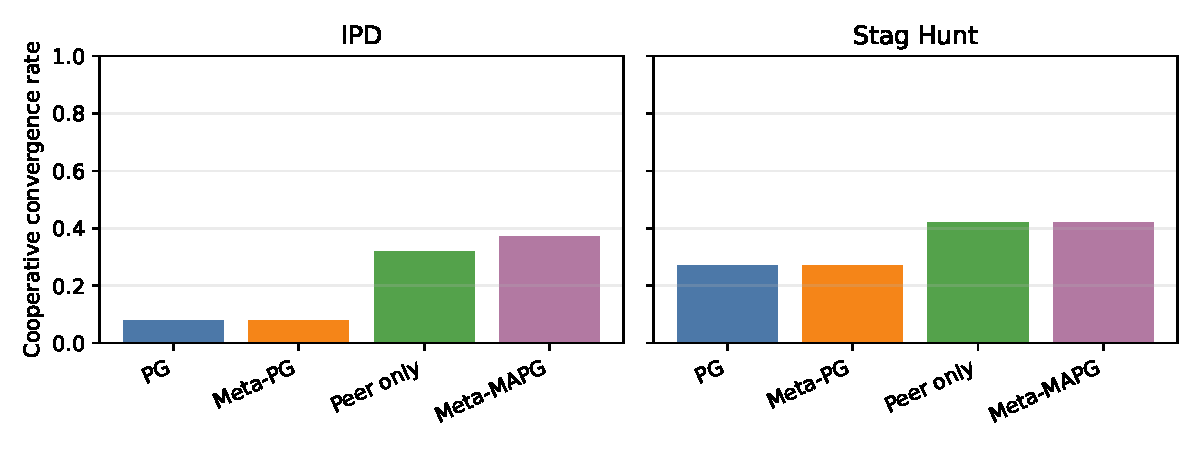
\includegraphics[width=\linewidth]{figures/ablation_success.pdf}
  \caption{Component ablation with Wilson $95\%$ confidence intervals over $100$ seeds. Peer-aware methods (peer-only, Meta-MAPG) are separated from non-peer methods (PG, Meta-PG) by non-overlapping CIs in both games, so the peer-learning effect is statistically significant. Peer-only and full Meta-MAPG are not distinguishable within CIs, so the figure does not claim strict dominance of the full method; it isolates that the peer-learning term is the component that changes cooperative outcomes.}
  \label{fig:ablation}
\end{figure}

\begin{figure}[t]
  \centering
  \includegraphics[width=\linewidth]{figures/basin_trajectories}
  \caption{Basin geometry and dynamics in Stag Hunt. Background shading is the empirical basin map on a $21\times21$ grid of initial cooperation probabilities (lavender = converges to the payoff-dominant equilibrium, cream = converges to the risk-dominant equilibrium). The dashed contour is the $0.5$-success level set of the smoothed basin indicator, i.e.\ the empirical separatrix. Overlaid trajectories show joint cooperation evolution from a $5\times5$ sub-grid of initialisations; green curves land above the frontier, red curves fall below. Under Meta-MAPG the frontier is pushed left and down: the certified basin grows from $27.0\%$ of the grid under PG to $42.6\%$, consistent with \cref{prop:basin}. This is not a convergence proof; it is the geometric bridge between the stochastic-approximation theorem and the restart-efficiency gains.}
  \label{fig:basin-traj}
\end{figure}

\begin{figure}[t]
  \centering
  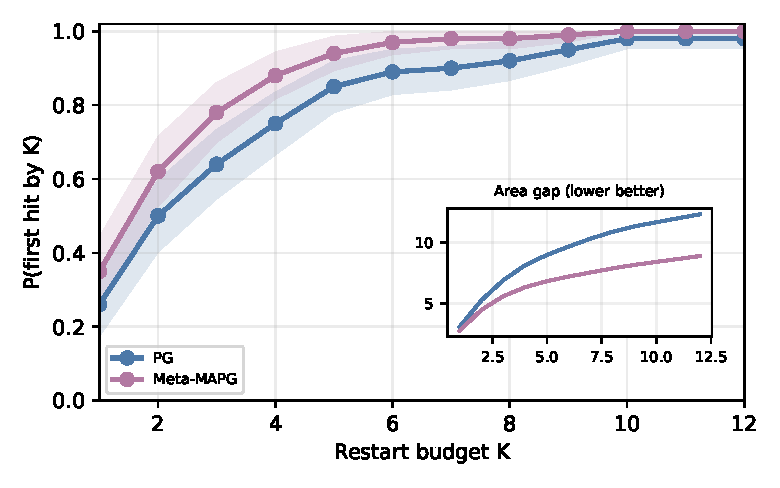
\includegraphics[width=\linewidth]{figures/restart_selection.pdf}
  \caption{Restart budget as an equilibrium-selection mechanism in Stag Hunt. For paired restart initialisations, we plot the probability that the payoff-dominant equilibrium has been discovered by budget $K$; bands show 95\% confidence intervals over seeds. The inset shows the cumulative area above the best-welfare curve, $\sum_{k\le K}(8-W_k)$, where lower is better. Meta-MAPG reaches the payoff-dominant basin with smaller restart budgets, consistent with opponent-aware shaping improving basin entry.}
  \label{fig:restart}
\end{figure}

\begin{figure}[t]
  \centering
  \includegraphics[width=\linewidth]{figures/peer_sweep}
  \caption{Peer-shaping sweep on Stag Hunt. Left: fraction of $11\times 11$ initial-policy grid points that converge to the payoff-dominant basin, as a function of the peer-shaping coefficient $\lambda$. The rate grows monotonically from the PG baseline ($\lambda=0$, $29.8\%$) to $62.8\%$ at $\lambda=5$, approximately linearly for small $\lambda$ as predicted by the certified-radius scaling $\rho_\lambda\gtrsim\rho_0+\lambda\mu_M/(2L)$ of \cref{prop:basin}. Right: mean first-hit step, conditional on eventual success, as a function of $\lambda$; basin-entry horizon contracts from $\approx 25$ steps to $\approx 20$ steps, consistent with \cref{cor:speedup}.}
  \label{fig:peer-sweep}
\end{figure}

\begin{figure}[t]
  \centering
  \includegraphics[width=\linewidth]{figures/annealing_ablation}
  \caption{Two-phase schedule vs constant shaping in Stag Hunt ($80$ seeds, $260$ steps, $\lambda_c=1.5$). Left: cooperative success rate. PG reaches $31\%$, constant-shaping Meta-MAPG reaches $41\%$, and the two-phase schedule of \cref{thm:two-phase} reaches $43\%$, showing that annealing to recover Nash consistency does not degrade empirical basin entry. Right: shaping schedule $\lambda_n$ versus step; the dotted vertical line is the phase-1/phase-2 boundary $N_0=100$. This is the only experiment that runs a genuinely annealed schedule rather than constant $\lambda$.}
  \label{fig:annealing}
\end{figure}

\begin{table}[t]
  \centering
  \caption{Main 100-seed summary. Cooperative success uses a minimum initial-state cooperation threshold of $0.82$. Restart entries are shown only for PG and Meta-MAPG because the restart experiment isolates the base-flow versus full opponent-aware comparison; the remaining variants are used for component ablation.}
  \label{tab:results}
  \resizebox{\linewidth}{!}{\begin{tabular}{llccc}\toprule
Game & Method & Ablation success & Restart success & Restarts \\\midrule
stag hunt & PG & 27\% & 100\% & 1.71 \\
stag hunt & Meta-PG & 27\% & -- & -- \\
stag hunt & Peer only & 42\% & -- & -- \\
stag hunt & Meta-MAPG & 42\% & 100\% & 1.24 \\
ipd & PG & 8\% & 51\% & 8.68 \\
ipd & Meta-PG & 8\% & -- & -- \\
ipd & Peer only & 32\% & -- & -- \\
ipd & Meta-MAPG & 37\% & 100\% & 2.13 \\
\bottomrule
\end{tabular}
}
\end{table}

The empirical claims are modest. The ablation primarily shows that peer-learning terms matter; it does not prove full Meta-MAPG dominates every LOLA-style variant in every game. The trajectory visualisation is finite-time mechanism evidence: it shows that opponent-aware shaping modifies the local flow in the same region where the basin map changes. The restart-budget, basin, and peer-sweep experiments are the direct support for \cref{thm:two-phase,thm:restart,prop:basin,cor:speedup}: restarts turn local convergence into equilibrium search, opponent-aware shaping improves that search by increasing the measured cooperative basin and first-passage probability in Stag Hunt, and \cref{fig:peer-sweep} shows the basin rate growing approximately linearly in $\lambda$ for small $\lambda$ with a corresponding contraction of the first-hit horizon, consistent with the certified-radius and basin-entry bounds. The annealing ablation in \cref{fig:annealing} is the one experiment that actually runs the two-phase schedule of \cref{thm:two-phase} rather than constant shaping; it shows that switching to annealed shaping after $N_0$ steps preserves or slightly improves cooperative success, so the annealed theorem is not paid for with empirical performance. The older restart-count statistic is retained in \cref{tab:results}. The estimator sanity check in \cref{app:sanity} is not a proof of \cref{as:decomp}; it is an implementation check that the sample estimator behaves in the predicted direction as batch size increases.

\section{Discussion}

The result is local before it is global. Meta-MAPG inherits Giannou et al.'s stable-Nash theory only inside attracting neighbourhoods and only after the estimator has been written in stochastic-approximation form. The two-phase theorem makes the algorithmic role of shaping explicit: constant shaping helps with basin entry, while annealing restores the original Nash target for asymptotic convergence. Restarts remove dependence on a particular initialisation and allow search across equilibrium basins; selecting the best discovered endpoint then turns restart budget into a simple equilibrium-selection mechanism. Its expected complexity depends on the basin probability $p_\rho$, so opponent-aware shaping helps only when it increases this probability.

The assumptions are substantive. The Meta-MAPG estimator must have bounded conditional variance, truncation schedules must make unroll bias summable, and asymptotic shaping must be Nash-consistent. Constant shaping is useful for basin geometry and finite-time behaviour, but in general-sum games a constant peer term can move the limiting fixed points. This is why the theorem separates annealed convergence from constant-shaping basin diagnostics.

The experiments are illustrative rather than definitive. They use matrix and tabular stochastic games because those are the settings in which the theorem's objects can be measured cleanly. Naive random restarts also degrade with dimension: the worst-case mass of a radius-$\rho$ basin inside a radius-$R$ search region scales like $(\rho/R)^d$. Extending the same decomposition to deep MARL therefore requires better variance control, opponent modeling, automatic differentiation through longer unrolls, and structured restart distributions such as warm starts around high-welfare policies, for example with DiCE-style estimators \citep{foerster2018dice}. The main point is narrower than a general deep-MARL convergence claim: opponent-aware gradients can be analysed as stochastic-approximation processes, and basin-entry efficiency is the right global metric when the underlying convergence theorem is local.

This paper does not claim unconditional convergence of arbitrary opponent-aware learning in deep MARL. It shows that finite-unroll Meta-MAPG can be analysed within classical stochastic approximation under boundedness, smoothness, Nash-consistency, and summability conditions, and that local convergence can be globalised by independent restarts when local basin mass is positive.

\appendix

\section{Detailed Estimator Decomposition}\label{app:decomp}

For a sampled trajectory $\tau$, write $S_i(\tau)=\nabla_{\phi_i}\log p_\phi(\tau)$ and $H_i(\tau)=\nabla_{\phi_i}^2\log p_\phi(\tau)$. The base likelihood-ratio estimator is $R_i(\tau)S_i(\tau)$ \citep{williams1992simple,sutton2018reinforcement}. The one-step own-learning derivative follows from differentiating $J_i(\phi_i+\eta\nabla_{\phi_i}J_i,\phi_{-i})$:
\[
\nabla_{\phi_i}J_i+\eta\left[\nabla_{\phi_i}^2J_i\right]^\top\nabla_{\phi_i}J_i.
\]
The Hessian identity gives
\[
\nabla_{\phi_i}^2J_i
=\E\left[R_i(\tau)\left(S_i(\tau)S_i(\tau)^\top+H_i(\tau)\right)\right],
\]
which is the estimator used in the experiments.

For the peer term, let agent $j$ take one inner step $\phi_j'=\phi_j+\eta\nabla_{\phi_j}J_j$. Differentiating $J_i(\phi_i,\phi_j')$ with respect to $\phi_i$ contributes
\[
\eta\left[\nabla_{\phi_i}\nabla_{\phi_j}J_j\right]^\top\nabla_{\phi_j}J_i.
\]
The mixed likelihood-ratio identity gives
\[
\nabla_{\phi_i}\nabla_{\phi_j}J_j
=\E\left[R_j(\tau)S_j(\tau)S_i(\tau)^\top\right],
\]
which is the sample cross-score matrix used for the peer correction. Longer Meta-MAPG unrolls repeat this chain-rule structure across $L$ inner updates; bounded derivatives on $\K$ allow the omitted tail and finite-modeling error to be collected in $b_n$.

\section{Local Lyapunov Drift}\label{app:lyapunov}

We spell out the stochastic-approximation step used in \cref{lem:local}. Fix an SOS Nash equilibrium $\phi^\ast$ and a ball $\B_\rho=\{\phi:\|\phi-\phi^\ast\|\le\rho\}$ on which the effective field $F$ satisfies
\[
\langle F(\phi),\phi-\phi^\ast\rangle\le -\mu\|\phi-\phi^\ast\|^2 .
\]
Assume $F$ is locally Lipschitz on $\B_\rho$, the iterates remain in $\B_\rho$ up to the stopping time under consideration, and
\[
\begin{gathered}
g_n=F(\phi_n)+\xi_{n+1}+b_n,\\
\E[\xi_{n+1}\mid\F_n]=0,\qquad
\E[\|\xi_{n+1}\|^2\mid\F_n]\le\sigma^2,
\end{gathered}
\]
with $\|b_n\|\le\beta_n$ and $\sum_n\alpha_n\beta_n<\infty$.

Let $V_n=\|\phi_n-\phi^\ast\|^2$. Ignoring projection can only increase the right-hand side locally, and projection onto a convex compact set is non-expansive. Therefore,
\[
\begin{aligned}
\E[V_{n+1}\mid\F_n]
&\le V_n
   +2\alpha_n\E[\langle g_n,\phi_n-\phi^\ast\rangle\mid\F_n]\\
&\quad+\alpha_n^2\E[\|g_n\|^2\mid\F_n]\\
&\le (1-2\mu\alpha_n)V_n
   +2\alpha_n\beta_n\sqrt{V_n}\\
&\quad+\alpha_n^2\E[\|g_n\|^2\mid\F_n].
\end{aligned}
\]
Since $F$ is bounded on $\B_\rho$, say $\|F(\phi)\|\le C_F$, the quadratic term obeys
\[
\E[\|g_n\|^2\mid\F_n]\le
3(C_F^2+\beta_n^2+\sigma^2).
\]
Equivalently, after absorbing bounded constants,
\[
\begin{aligned}
\E[V_{n+1}\mid\F_n]
&\le (1-2\mu\alpha_n)V_n
   +2\alpha_n\beta_n\sqrt{V_n}\\
&\quad+C\alpha_n^2(C_F^2+\sigma^2+\beta_n^2).
\end{aligned}
\]
Using $2\alpha_n\beta_n\sqrt{V_n}\le \alpha_n\beta_n(1+V_n)$ gives the Robbins--Siegmund form
\[
\E[V_{n+1}\mid\F_n]\le (1-a_n)V_n+\eta_n,
\]
where $\sum_n a_n=\infty$ and $\sum_n\eta_n<\infty$ for sufficiently large $n$. Robbins--Siegmund then implies $V_n\to V_\infty$ almost surely and $\sum_n a_nV_n<\infty$; since $\sum_n a_n=\infty$, we obtain $V_\infty=0$. Thus $\phi_n\to\phi^\ast$ almost surely on the local event.

\section{Proof of Proposition~\ref{prop:basin}}\label{app:prop-basin}

We prove the two parts separately.

\paragraph{Linearised drift bound.}
By assumption $v,M\in C^1$ in a neighbourhood of $\phi^\ast$. Both $J_v$ and $J_M$ are real matrices; their symmetric parts $\operatorname{sym}(A):=(A+A^\top)/2$ are Hermitian. By definition, $-\lambda_{\max}(\operatorname{sym}(J_v))=\mu$ (the SOS margin) and $-\lambda_{\max}(\operatorname{sym}(J_M))=\mu_M$. For any $\lambda\ge 0$,
\[
\operatorname{sym}(J_\lambda)=\operatorname{sym}(J_v)+\lambda\operatorname{sym}(J_M),
\]
which is Hermitian. Weyl's inequality for Hermitian matrices gives
\[
\lambda_{\max}\!\bigl(\operatorname{sym}(J_\lambda)\bigr)\le \lambda_{\max}\!\bigl(\operatorname{sym}(J_v)\bigr)+\lambda\,\lambda_{\max}\!\bigl(\operatorname{sym}(J_M)\bigr).
\]
Negating both sides yields \eqref{eq:weyl}. The bound is exact, not asymptotic, and requires no smallness condition on $\lambda$.

\paragraph{Certified radius.}
Let $\mu_\lambda:=\mu+\lambda\mu_M$. Fix $\phi\in\B_\rho(\phi^\ast)$ and write $x:=\phi-\phi^\ast$. Because $F_\lambda(\phi^\ast)=v(\phi^\ast)+\lambda M(\phi^\ast)=0$ and $M(\phi^\ast)=0$, Taylor's theorem with the integral remainder gives
\[
F_\lambda(\phi)=J_\lambda x+R_\lambda(x),
\qquad
\|R_\lambda(x)\|\le \tfrac{1}{2}L_\lambda\|x\|^2,
\]
where $L_\lambda$ is the Lipschitz constant of $DF_\lambda$ on $\B_\rho(\phi^\ast)$. Taking inner products,
\[
\langle F_\lambda(\phi),x\rangle
=\langle J_\lambda x,x\rangle+\langle R_\lambda(x),x\rangle.
\]
The first term obeys $\langle J_\lambda x,x\rangle=x^\top\operatorname{sym}(J_\lambda)x\le -\mu_\lambda\|x\|^2$ by the Rayleigh quotient and \eqref{eq:weyl}. The remainder obeys $|\langle R_\lambda(x),x\rangle|\le \tfrac{1}{2}L_\lambda\|x\|^3$. Therefore
\[
\langle F_\lambda(\phi),\phi-\phi^\ast\rangle\le -\mu_\lambda\|x\|^2+\tfrac{1}{2}L_\lambda\|x\|^3.
\]
Whenever $\|x\|\le \rho_\lambda:=\mu_\lambda/(2L_\lambda)$, the cubic term is at most $(\mu_\lambda/4)\|x\|^2$, so
\[
\langle F_\lambda(\phi),\phi-\phi^\ast\rangle\le -\tfrac{3}{4}\mu_\lambda\|x\|^2\le -\tfrac{1}{2}\mu_\lambda\|x\|^2.
\]
This proves the stated SOS drift on $\B_{\rho_\lambda}(\phi^\ast)$. $\square$

\section{Proof of Theorem~\ref{thm:two-phase}}\label{app:thm-twophase}

Write $V_n=\|\phi_n-\phi^\ast\|^2$ and let $\tau:=\inf\{n\le N_0:\phi_n\notin\B_\rho\}$ with $\tau=N_0+1$ if the iterates never leave. On the event $\{n<\tau\}$ the phase-1 drift of \cref{prop:basin} applies with constant $\mu_{\lambda_c}$.

\paragraph{Step 1: one-step drift.}
On $\{n<\tau\}$, by \cref{as:decomp} and the phase-1 drift bound,
\[
\begin{aligned}
\E[V_{n+1}\mid\F_n]
&=\E\!\left[\|\phi_n-\phi^\ast+\alpha_0 g_n\|^2\mid\F_n\right]\\
&=V_n+2\alpha_0\langle F_{\lambda_c}(\phi_n),\phi_n-\phi^\ast\rangle\\
&\quad+2\alpha_0\langle b_n,\phi_n-\phi^\ast\rangle+\alpha_0^2\E[\|g_n\|^2\mid\F_n]\\
&\le V_n-2\alpha_0\mu_{\lambda_c}V_n
+2\alpha_0\beta_0\sqrt{V_n}+\alpha_0^2 G^2,
\end{aligned}
\]
where $G^2:=3(C_{F_{\lambda_c}}^2+\beta_0^2+\sigma^2)$ is a uniform bound on the conditional second moment of $g_n$ (with $C_{F_{\lambda_c}}$ the sup-norm of $F_{\lambda_c}$ on $\B_\rho$). Applying $2a b\le \eta a^2+\eta^{-1}b^2$ with $a=\sqrt{V_n}$, $b=\beta_0$, and $\eta=\mu_{\lambda_c}$,
\[
\E[V_{n+1}\mid\F_n]\le (1-\mu_{\lambda_c}\alpha_0)V_n
+\frac{\alpha_0\beta_0^2}{\mu_{\lambda_c}}+\alpha_0^2 G^2.
\]

\paragraph{Step 2: unconditional recursion on the stopped process.}
Define the stopped sequence $\tilde V_n:=V_{n\wedge\tau}$. The drift bound and the fact that $\tilde V_{n+1}=\tilde V_n$ on $\{n\ge\tau\}$ give
\[
\E[\tilde V_{n+1}]\le (1-\mu_{\lambda_c}\alpha_0)\E[\tilde V_n]+c_1,
\qquad c_1:=\frac{\alpha_0\beta_0^2}{\mu_{\lambda_c}}+\alpha_0^2 G^2.
\]
Iterating,
\[
\E[\tilde V_{N_0}]\le (1-\mu_{\lambda_c}\alpha_0)^{N_0}V_0+\frac{c_1}{\mu_{\lambda_c}\alpha_0}.
\]
Using $(1-x)^k\le e^{-xk}$ for $x\in[0,1]$,
\[
\E[\tilde V_{N_0}]\le V_0\,e^{-\mu_{\lambda_c}\alpha_0 N_0}+\frac{\beta_0^2}{\mu_{\lambda_c}^2}+\frac{\alpha_0 G^2}{\mu_{\lambda_c}}.
\]

\paragraph{Step 3: Markov's inequality.}
If $\phi_{N_0}\notin\B_{\rho/2}$ and $\tau>N_0$, then $V_{N_0}\ge (\rho/2)^2$. If $\tau\le N_0$, by continuity of trajectories (or by projection onto $\K$) the iterate at time $\tau$ already lies outside $\B_\rho$, and in particular $V_\tau\ge \rho^2\ge (\rho/2)^2$; $\tilde V_{N_0}=V_\tau$ in that case. Hence in both cases $\tilde V_{N_0}\ge (\rho/2)^2$. Therefore
\[
\Pr(\phi_{N_0}\notin\B_{\rho/2}\mid \phi_0\in\B_\rho)
\le \Pr(\tilde V_{N_0}\ge (\rho/2)^2)
\le \frac{4\E[\tilde V_{N_0}]}{\rho^2}.
\]
Combining with Step 2,
\[
\Pr(\phi_{N_0}\notin\B_{\rho/2}\mid\phi_0\in\B_\rho)
\le \frac{4}{\rho^2}\!\left(V_0 e^{-\mu_{\lambda_c}\alpha_0 N_0}+C\alpha_0(\beta_0^2+\alpha_0\sigma^2)\right),
\]
for a constant $C$ depending on $\mu_{\lambda_c}$, $C_{F_{\lambda_c}}$.

\paragraph{Step 4: choice of $N_0$.}
Given a target $\delta\in(0,1)$, set
\[
N_0=\left\lceil\frac{1}{\mu_{\lambda_c}\alpha_0}\log\!\frac{8V_0}{\delta\rho^2}\right\rceil,
\qquad \alpha_0\le \frac{\delta\rho^2}{8C(\beta_0^2+\sigma^2)}.
\]
Each summand in Step 3 is then at most $\delta/2$, so the total failure probability is at most $\delta$.

\paragraph{Step 5: phase 2.}
Conditional on $\phi_{N_0}\in\B_{\rho/2}$, the subsequent recursion uses $\alpha_n=\alpha_0 n^{-p}$ and $\lambda_n=\lambda_c n^{-q}$ with $1/2<p\le 1$ and $q>1-p$, so $\sum_n\alpha_n=\infty$, $\sum_n\alpha_n^2<\infty$, and $\sum_n\alpha_n\lambda_n<\infty$ by direct integral comparison. Together with \cref{as:trunc,as:decomp,as:stable}, this satisfies the hypotheses of \cref{lem:local} on the event $\{\phi_{N_0}\in\B_{\rho/2}\}$. Conditional on this event, $\phi_n\to\phi^\ast$ almost surely. The total probability that the two-phase procedure converges in a single epoch is therefore at least $(1-\delta)\cdot 1=1-\delta$. $\square$

\section{Proof of Theorem~\ref{thm:restart}}\label{app:thm-restart}

Let $\F_k^{\mathrm{epoch}}$ denote the $\sigma$-algebra generated by epochs $1,\ldots,k-1$ (outcomes only; restart draws are independent by assumption). Let $A_k$ be the event that epoch $k$ starts in $\B_\rho$ and that the two-phase procedure of \cref{thm:two-phase} reaches phase 2 and converges within that epoch.

\paragraph{Step 1: per-epoch lower bound.}
Restart $k$ samples $\phi_0^{(k)}\sim\nu$ independently of $\F_k^{\mathrm{epoch}}$, so
\[
\Pr(\phi_0^{(k)}\in\B_\rho\mid\F_k^{\mathrm{epoch}})=\nu(\B_\rho)=p_\rho.
\]
Conditional on $\phi_0^{(k)}\in\B_\rho$, \cref{thm:two-phase} gives $\Pr(\text{epoch succeeds})\ge 1-\delta$. Therefore
\[
\Pr(A_k\mid\F_k^{\mathrm{epoch}})\ge p_\rho(1-\delta)=:p_\star>0.
\]

\paragraph{Step 2: geometric tail.}
Let $T:=\inf\{k\ge 1:A_k\text{ occurs}\}$. Then
\[
\Pr(T>k)=\E\!\left[\prod_{j=1}^k\mathbf{1}_{A_j^c}\right]
=\E\!\left[\E[\mathbf{1}_{A_k^c}\mid\F_k^{\mathrm{epoch}}]\prod_{j=1}^{k-1}\mathbf{1}_{A_j^c}\right].
\]
By Step 1, $\E[\mathbf{1}_{A_k^c}\mid\F_k^{\mathrm{epoch}}]\le 1-p_\star$ almost surely, so iterating,
\[
\Pr(T>k)\le (1-p_\star)^k.
\]
Hence $\Pr(T<\infty)=1$ and
\[
\E[T]=\sum_{k\ge 0}\Pr(T>k)\le \sum_{k\ge 0}(1-p_\star)^k=\frac{1}{p_\star}.
\]

\paragraph{Step 3: dimensional dependence.}
If $\nu$ is lower-bounded by density $m>0$ on a region containing $\B_\rho(\phi^\ast)$ in $\R^d$, then $p_\rho\ge m\,c_d\rho^d$ where $c_d=\pi^{d/2}/\Gamma(d/2+1)$ is the volume of the unit $d$-ball. Combined with the certified radius $\rho_\lambda\ge (\mu+\lambda\mu_M)/(2L_\lambda)$ from \cref{prop:basin}, the expected number of epochs obeys
\[
\E[T]\le \frac{1}{(1-\delta)m c_d}\!\left(\frac{2L_\lambda}{\mu+\lambda\mu_M}\right)^{\!d}.
\]
Shaping reduces the base of this dimensional factor whenever $\mu_M>0$; the overall worst-case dependence is still exponential in $d$, as discussed in \cref{sec:main}. $\square$

\section{Experiment Reproducibility}\label{app:repro}

Code, scripts, and plotting utilities for the experiments are available at \url{https://github.com/guernicastars/icml26_drafts}. The generated artifacts used in this paper are written under \texttt{artifacts/main}, including \texttt{ablation\_summary.csv}, \texttt{restart\_summary.csv}, \texttt{restart\_selection.csv}, \texttt{trajectory\_trace.csv}, \texttt{basin\_map.csv}, \texttt{estimator\_sanity.csv}, \texttt{peer\_sweep.csv}, and \texttt{annealing\_ablation.csv}. The implementation does not use exact gradients for learning updates; expected returns are computed only for logging and evaluation.

\section{Estimator Sanity Check}\label{app:sanity}

\begin{figure}[h]
  \centering
  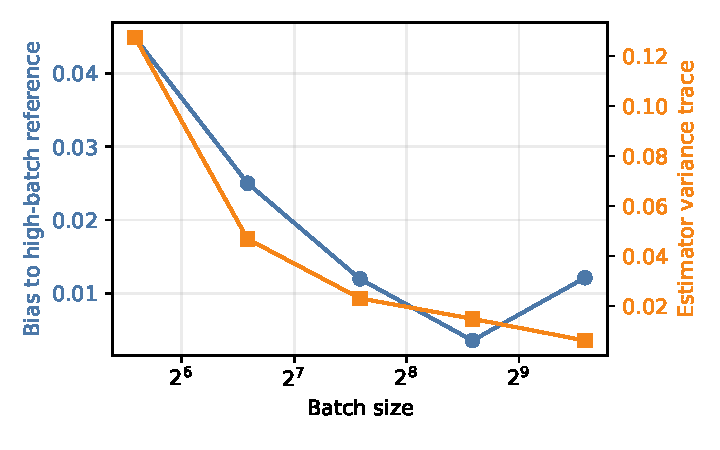
\includegraphics[width=0.78\linewidth]{figures/estimator_sanity.pdf}
  \caption{Estimator sanity check. At a fixed Stag Hunt parameter, the variance trace of the Meta-MAPG estimator decreases from $0.1272$ at batch size $48$ to $0.0062$ at batch size $768$. Bias is measured relative to a high-batch reference estimator, not an exact analytic gradient.}
  \label{fig:sanity}
\end{figure}

\bibliography{references}
\bibliographystyle{icml2026}

\end{document}
